\documentclass[11pt]{article}

\usepackage[T1]{fontenc}
\usepackage[utf8]{inputenc}
\usepackage{lmodern}
\usepackage{microtype}
\usepackage[a4paper,margin=24mm,headheight=16pt]{geometry}
\usepackage{amsmath,amssymb,mathtools}
\usepackage{booktabs,tabularx,longtable,array,multirow}
\usepackage{enumitem}
\usepackage{xcolor}
\usepackage{hyperref}
\usepackage{fancyhdr}
\usepackage{titlesec}
\usepackage{listings}
\usepackage{tikz}
\usetikzlibrary{arrows.meta,positioning,fit,shapes.geometric}

\definecolor{navy}{HTML}{15395B}
\definecolor{steel}{HTML}{4A6682}
\definecolor{pale}{HTML}{ECF3F8}
\definecolor{green}{HTML}{25633E}
\definecolor{greenpale}{HTML}{EAF5EE}
\definecolor{amber}{HTML}{7A5600}
\definecolor{amberpale}{HTML}{FFF4D6}
\definecolor{red}{HTML}{8D2B35}
\definecolor{redpale}{HTML}{FBECEE}
\definecolor{ink}{HTML}{202C38}

\hypersetup{
  colorlinks=true,
  linkcolor=navy,
  urlcolor=steel,
  citecolor=navy,
  pdftitle={Certification Audit of the Cone-Scheme Decision Procedure},
  pdfauthor={OpenAI Codex, under user direction},
  pdfsubject={The forall-PO-free fragment of ALCI-RCC5, its full-logic boundary, and related work}
}

\pagestyle{fancy}
\fancyhf{}
\fancyhead[L]{\small\color{steel}$\forall\mathsf{PO}$-free $\mathcal{ALCI}_{\mathrm{RCC5}}$}
\fancyhead[R]{\small\color{steel}Certification audit}
\fancyfoot[C]{\small\thepage}
\renewcommand{\headrulewidth}{0.4pt}

\titleformat{\section}{\Large\bfseries\color{navy}}{\thesection}{0.65em}{}
\titleformat{\subsection}{\large\bfseries\color{navy}}{\thesubsection}{0.65em}{}
\titleformat{\subsubsection}{\normalsize\bfseries\color{steel}}{\thesubsubsection}{0.65em}{}
\setlist[itemize]{leftmargin=1.6em,itemsep=0.25em,topsep=0.35em}
\setlist[enumerate]{leftmargin=1.8em,itemsep=0.25em,topsep=0.35em}
\setlength{\parindent}{0pt}
\setlength{\parskip}{0.55em}
\allowdisplaybreaks

\lstdefinelanguage{Lean}{
  morekeywords={theorem,def,structure,inductive,where,by,let,have,show,from,
    if,then,else,match,with,fun,forall,exists,namespace,end,import,open,
    instance,deriving,Decidable,Finite,Fintype,Prop,Type},
  sensitive=true,
  morecomment=[l]{--},
  morestring=[b]"
}
\lstset{
  language=Lean,
  basicstyle=\ttfamily\small,
  keywordstyle=\color{navy}\bfseries,
  commentstyle=\color{steel},
  stringstyle=\color{green},
  columns=fullflexible,
  keepspaces=true,
  breaklines=true,
  frame=single,
  rulecolor=\color{steel!40},
  backgroundcolor=\color{pale!55},
  xleftmargin=0.4em,
  xrightmargin=0.4em
}

\newcommand{\PP}{\mathsf{PP}}
\newcommand{\PPI}{\mathsf{PPI}}
\newcommand{\PO}{\mathsf{PO}}
\newcommand{\DR}{\mathsf{DR}}
\newcommand{\EQ}{\mathsf{EQ}}
\newcommand{\Ty}{\mathsf{Ty}}
\newcommand{\Cl}{\mathsf{Cl}^{+}}
\newcommand{\Sat}{\mathsf{Sat}}
\newcommand{\BoxR}[2]{[\mathsf{#1}]#2}
\newcommand{\statusbox}[3]{%
  \begin{center}
  \fcolorbox{#1}{#2}{\begin{minipage}{0.91\linewidth}\textbf{#3}\end{minipage}}
  \end{center}}
\newcommand{\code}[1]{\texttt{#1}}
\newcommand{\sha}[2]{{\scriptsize\ttfamily #1\linebreak #2}}

\begin{document}

\pagenumbering{gobble}
\begin{titlepage}
\thispagestyle{empty}
\vspace*{1.25cm}
{\color{navy}\rule{\linewidth}{1.2pt}}\\[1.0cm]
{\huge\bfseries\color{navy}Certification Audit of the\\[0.18cm]
Cone-Scheme Decision Procedure\par}
\vspace{0.55cm}
{\Large\color{steel}The $\forall\PO$-free fragment of
$\mathcal{ALCI}_{\mathrm{RCC5}}$, its full-logic boundary,\\
and its closest related work\par}
\vspace{1.15cm}

\begin{center}
\renewcommand{\arraystretch}{1.25}
\begin{tabularx}{0.92\linewidth}{>{\bfseries}rX}
Artifact reviewed: & \code{cone\_scheme\_attack.zip}, supplied 2026-08-28 \\
Report date: & 2026-08-29 \\
Technical author: & OpenAI Codex, under the user's direction \\
Formal target: & already-NNF concepts, abstract composition-table RCC5 semantics \\
Verdict: & core proof chain survives cold attack; release certification is incomplete
\end{tabularx}
\end{center}

\vfill
\begin{center}
\fcolorbox{navy}{pale}{%
\begin{minipage}{0.88\linewidth}
\textbf{Bottom line.}
The supplied Lean source contains a coherent finite greatest-fixed-point decision
procedure and a fresh-occurrence soundness construction for the entire stated
$\forall\PO$-free, mixed-quadrant fragment. No mathematical counterexample was
found. This is not yet a release-grade certification: the source was not rebuilt in
the present runtime, and the raw-syntax normalization, concrete-region adequacy
bridge, pinned toolchain, capstone axiom transcript, and full regression gate are
absent. The argument does not presently prove decidability of full
$\mathcal{ALCI}_{\mathrm{RCC5}}$; universal $\PO$ restrictions create a global
all-pairs compatibility problem that the local cone signatures do not record.
\end{minipage}}
\end{center}
\vspace{0.8cm}
{\color{navy}\rule{\linewidth}{1.2pt}}
\end{titlepage}

\pagenumbering{roman}
\begin{abstract}
This report audits a claimed Lean decision procedure for the fragment of
$\mathcal{ALCI}_{\mathrm{RCC5}}$ in negation normal form containing no universal
$\PO$ restriction. The procedure enumerates finite cone signatures, removes
unsupported signatures by a monotone reductive operator, and unfolds any surviving
signature into an infinite fresh-occurrence model. The audit traces the exact Lean
declarations from syntax and semantics through completeness, ordered-disjoint
geometry, the truth lemma, fixed-round correctness, and the final
\code{Decidable} theorem. It independently reruns the supplied Python probes and
separates their evidential value from the Lean theorem.

The core result appears mathematically sound for the semantics actually formalized:
carrier-polymorphic frames whose five RCC5 atoms satisfy strong equality and the
abstract composition table. The present packet does not formally identify these
frames with a conventional nonempty-region semantics, and it accepts already-NNF
syntax only. The report therefore assigns a qualified rather than final
certification label.

An authorial generalization analysis identifies the exact failure at full logic.
In the unfolding, every pair that is neither ordered nor disjoint is labelled
$\PO$. A formula $\forall\PO.D$ consequently constrains arbitrary residual pairs,
including cousins in unrelated generated branches. The current proof disposes of
this case solely by the fragment hypothesis. A conditional PO-safe extension is
straightforward, but full decidability requires new finite global interface
machinery or a different automata argument. A staged Lean research plan and explicit
go/no-go gates are given. Finally, the report compares the work with RCC constraint
networks, composition-based spatial description logics, modal logics of topological
relations, concrete-domain systems, type elimination, and unravelling. The finite
GFP and fresh-witness ingredients are standard; no source was identified for the
specific lower-spectrum cone signatures plus protected residual-PO unfolding or for
this exact Lean result.
\end{abstract}

\setcounter{tocdepth}{2}
\tableofcontents
\clearpage
\pagenumbering{arabic}

\section{Executive assessment}

\statusbox{green}{greenpale}{Within the explicitly formalized abstract semantics,
the packet contains a genuine end-to-end decision theorem for every already-NNF
concept satisfying \code{POFree}. The cold attack found no counterexample and no
degenerate definition in the capstone route.}

\statusbox{amber}{amberpale}{The appropriate public label is
``substantively machine-formalized, independently source-audited, not yet
reproducibly release-certified.'' A clean Lean 4.32.0 rebuild and several semantic
and packaging obligations remain.}

The capstone declaration is:
\begin{lstlisting}
def decidableSat_cone (C0 : Concept) (hpo : POFree C0) :
    Decidable (Satisfiable C0)
\end{lstlisting}
It has no oracle or semantic premise. The decision is a finite list computation;
the model construction occurs only in its correctness proof. The strongest honest
reading is therefore:
\[
  \forall C_0\in\mathsf{Concept}_{\mathrm{NNF}},\quad
  \mathsf{POFree}(C_0)\Longrightarrow
  \mathsf{Decidable}\bigl(\mathsf{Satisfiable}_{\mathrm{absRCC5}}(C_0)\bigr).
\]

The audit distinguishes four levels that should not be collapsed.

\begin{center}
\renewcommand{\arraystretch}{1.22}
\begin{tabularx}{\linewidth}{>{\bfseries}p{0.19\linewidth}p{0.18\linewidth}X}
\toprule
Level & Status & Meaning \\
\midrule
Mathematical architecture & Passed cold attack & The finite GFP, source-model
post-fixed point, occurrence geometry, and one-way truth lemma fit together. \\
Lean source chain & Present & All principal declarations through
\code{decidableSat\_cone} occur in the supplied source; static scans found no
declaration-form axiom, \code{sorry}, \code{opaque}, or \code{unsafe}. \\
Independent build & Not performed & The present runtime has no Lean executable.
The claimed Lean 4.32.0 build and axiom footprint were not reproduced. \\
External adequacy & Partial & The theorem targets abstract composition-table frames
and already-NNF syntax. A raw-syntax theorem and a satisfaction-preserving bridge to
ordinary set/region semantics are not packaged. \\
\bottomrule
\end{tabularx}
\end{center}

\subsection{Answer to the full-logic question}

The proof generalizes \emph{structurally} but not yet \emph{theoremically} to full
$\mathcal{ALCI}_{\mathrm{RCC5}}$. All finite-control, completeness, order, disjointness,
existential, and non-PO universal machinery remains useful. One branch of the Lean
truth lemma is missing: the case for $\forall\PO.D$. Yet that single branch is not a
local lemma. It asks that every residual PO pair in an infinite unfolding satisfy a
two-sided type-compatibility condition. Pairs of separately born branches are not
visible to either birth transition, so the current state cannot certify them.

The present proof therefore extends immediately only to instances equipped with an
additional certificate that every residual PO pair is safe. It also extends to simple
sufficient subfragments in which every PO-box body is globally true at all surviving
types. It does not establish decidability for arbitrary $\forall\PO$ formulas.

\subsection{Answer to the novelty question}

The responsible novelty claim is narrow. Type enumeration, monotone elimination,
greatest fixed points, unravelling, and fresh witnesses are standard modal and
description-logic methods. RCC5 composition and ordered/disjoint region
representations are also established ideas. The apparently new contribution is their
specific combination:
\begin{itemize}
  \item a finite signature $(T,S)$ consisting of a local support type and its possible
  strict-lower type spectrum;
  \item an inclusive-cone compatibility test that makes vertical and downward-DR
  propagation compositional;
  \item a monotone reductive elimination whose real-model signatures form a
  post-fixed point; and
  \item an infinite fresh-occurrence ordered-disjoint unfolding in which PO is
  residual and is sound precisely because universal PO boxes are absent.
\end{itemize}
No checked source was found that states the exact $\forall\PO$-free theorem, uses this
combination, or mechanizes it in Lean. This is evidence for novelty, not a universal
priority guarantee; unpublished material or differently named equivalent machinery
could still exist.

\section{Exact formal scope}

\subsection{Syntax and semantics in the artifact}

The \code{Concept} datatype is already in negation normal form. Atomic concept names
and their negative literals are primitive; conjunction, disjunction, existential role
restrictions, and universal role restrictions are constructors. The five roles are
\[
  \mathsf{RCC5}=\{\EQ,\DR,\PO,\PP,\PPI\}.
\]
The interpretation is carrier-polymorphic. \code{RCC5Interp} enforces strong identity
for $\EQ$, converse behavior, exhaustiveness/exclusivity, and the abstract RCC5
composition table. \code{Satisfiable C0} quantifies over a carrier, an interpretation,
an RCC5 proof, and a designated domain point satisfying $C_0$.

This is a legitimate and useful semantic target. It must nevertheless be named. A
conventional spatial presentation begins with nonempty regions and defines $\PP$ by
proper inclusion, $\DR$ by disjointness, $\PO$ by nonempty intersection without
inclusion, and $\PPI$ by converse inclusion. The separate
\code{RCC5NormalForm.lean} develops a canonical set representation for an
ordered-disjoint structure, including inclusion, injectivity, and disjointness facts.
It does not yet export the five concrete relations and prove a bidirectional
satisfaction-preservation theorem connecting that representation to
\code{POFreeLift.Satisfiable}.

\subsection{What \code{POFree} means}

\code{POFree C0} recursively excludes every universal restriction with role $\PO$.
Existential PO demands remain allowed and are central to the mixed-quadrant theorem.
The closure lemmas propagate the absence of a PO box to all relevant subformulas.
Thus the result is not a PO-free logic: it is only $\forall\PO$-free.

The distinction is the entire proof boundary. The soundness construction can always
birth a fresh PO witness for $\exists\PO.D$. What it cannot locally check is a box
$\forall\PO.D$ against every unrelated pair that later becomes residual PO.

\subsection{What is not yet included}

The packet does not currently provide:
\begin{itemize}
  \item a raw concept syntax, an NNF transformation, or a theorem
  $\mathsf{sat}(C)\leftrightarrow\mathsf{sat}(\mathsf{nnf}(C))$;
  \item a formal equivalence to a conventional nonempty-region/set semantics;
  \item a public Boolean \code{coneSatCoreB} and three-way wrapper that returns
  \code{outOfScope} on concepts containing a universal PO restriction;
  \item a formal closed expression for the advertised finite-state/complexity bound;
  or
  \item general TBoxes, nominals, number restrictions, role hierarchies beyond the
  fixed RCC5 table, or the full $\forall\PO$ language.
\end{itemize}

\section{Why the cone scheme works}

\subsection{Finite control, infinite model}

Let $\Cl(C_0)$ be the finite positive closure and let $\Ty(C_0)$ be the enumerated
support types. A cone signature is
\[
  q=(T,S),\qquad T\in\Ty(C_0),\quad S\subseteq\Ty(C_0),
\]
where $T$ is the local type and $S$ is the spectrum of types that may occur strictly
below the point in the generated proper-part order. The initial list
$\mathsf{sigStatic}(C_0)$ contains exactly the finitely checkable local candidates.

For a relation demand $(r,D)$ of $T$, a target signature must carry $D$ and satisfy
\code{compatB}. Compatibility expresses the singleton composition consequences that
must cross the birth edge. For example, proper-part edges transport relevant universal
information into a whole cone, and a DR cut must remain disjoint from every descendant
on both sides. PO births are protected from later being turned into order or
disjointness.

Define the elimination operator
\[
  \Phi(X)=\{q\in X:\text{every demand of }q\text{ has a compatible target in }X\}.
\]
It is reductive and monotone. Iteration from $\mathsf{sigStatic}(C_0)$ reaches its
greatest fixed point in at most the length of that list. Acceptance asks whether a
surviving signature contains $C_0$ in its local type.

\subsection{Completeness as a post-fixed-point argument}

Given a genuine source model and a point $x$, form its exact signature:
the local closure type realized at $x$, together with the set of realized types strictly
below $x$. The artifact proves that exact signatures are static and that every real
witness induces a compatible transition. Consequently the finite list of signatures
realized in the model satisfies
\[
  X_{M}\subseteq \Phi(X_{M}).
\]
By greatestness, $X_M$ survives every elimination round. A source point satisfying
$C_0$ therefore yields an accepting survivor. No finite submodel or quotient must be
extracted; this avoids the cycle and shared-witness failures of earlier approaches.

\subsection{Soundness by fresh occurrences}

Starting from a surviving signature, the construction recursively chooses a target for
each demand. Every non-EQ demand creates a new occurrence even if its finite control
signature has appeared before. The carrier is the subtype of generated finite demand
words. Control may loop while domain points remain distinct.

The generated geometry is described by a strict order $<$ and a symmetric disjointness
relation $\#$:
\begin{itemize}
  \item vertical PP/PPI births generate $<$ and its transitive closure;
  \item DR births generate cuts whose descendant cones are placed in $\#$;
  \item order and disjointness are proved incompatible; and
  \item any unequal pair that is neither comparable nor disjoint receives residual PO.
\end{itemize}
The resulting five relations satisfy the abstract RCC5 frame axioms. An induction on
concept structure then proves that every formula in an occurrence label is true there.
All existential cases use the corresponding fresh child. The $\forall\PP$,
$\forall\PPI$, $\forall\DR$, and $\forall\EQ$ cases use the cone and label propagation
lemmas. The $\forall\PO$ branch is impossible by \code{POFree}.

\begin{center}
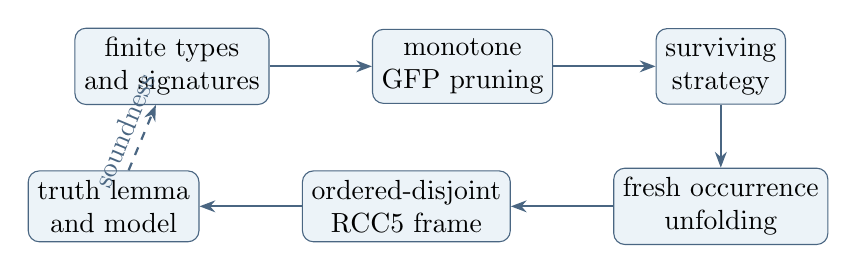
\begin{tikzpicture}[
  node distance=8mm and 13mm,
  box/.style={draw=steel,rounded corners,fill=pale,align=center,minimum height=8mm},
  arr/.style={-{Stealth[length=2mm]},thick,color=steel}
]
\node[box] (types) {finite types\\and signatures};
\node[box,right=of types] (gfp) {monotone\\GFP pruning};
\node[box,right=of gfp] (strategy) {surviving\\strategy};
\node[box,below=of strategy] (occ) {fresh occurrence\\unfolding};
\node[box,left=of occ] (frame) {ordered-disjoint\\RCC5 frame};
\node[box,left=of frame] (truth) {truth lemma\\and model};
\draw[arr] (types) -- (gfp);
\draw[arr] (gfp) -- (strategy);
\draw[arr] (strategy) -- (occ);
\draw[arr] (occ) -- (frame);
\draw[arr] (frame) -- (truth);
\draw[arr,dashed] (truth) -- node[above,sloped,align=center]{soundness} (types);
\end{tikzpicture}
\end{center}

\subsection{The decision theorem}

The final proof avoids noncomputably choosing a stabilization round. It proves that
iteration exactly $|\mathsf{sigStatic}(C_0)|$ times is already fixed, establishes
\[
\mathsf{Satisfiable}(C_0)\quad\Longleftrightarrow\quad
\exists q\in\Phi^{|\mathsf{sigStatic}(C_0)|}(\mathsf{sigStatic}(C_0)),
\;C_0\in q.1,
\]
and transfers the decidability of the finite right-hand side to satisfiability.

\section{Lean theorem-chain audit}

The source is a 44,375-line monolith containing several retired approaches before the
cone scheme. The relevant capstone begins near line 41,861. Table~\ref{tab:chain}
records the declarations that actually carry the result. Line numbers refer to the
supplied \code{lean/POFreeLift.lean}.

\begin{longtable}{>{\raggedright\arraybackslash}p{0.18\linewidth}
                  >{\raggedright\arraybackslash}p{0.36\linewidth}
                  >{\raggedright\arraybackslash}p{0.34\linewidth}}
\caption{Principal Lean declarations in the cone-scheme chain.}\label{tab:chain}\\
\toprule
Layer and lines & Declarations & Audit reading \\
\midrule
\endfirsthead
\toprule
Layer and lines & Declarations & Audit reading \\
\midrule
\endhead
Syntax/semantics, 378--420 & \code{Concept}, \code{Interp}, \code{sat},
\code{RCC5Interp}, \code{Satisfiable} & Already-NNF syntax and abstract,
carrier-polymorphic RCC5 composition-table semantics. \\
Fragment, 1143--1177 & \code{POFree}, \code{pofreeB}, \code{pofreeB\_iff} &
Syntactic exclusion of every universal PO restriction and Boolean reflection. \\
Finite controls, 41861--41936 & \code{Sig}, \code{supportB}, \code{sigOkB},
\code{sigStatic}, \code{compatB}, \code{sigDemands} & Enumerated local types,
lower spectra, and demand transitions. \\
Elimination, 41937--41976 & \code{pruneSig}, \code{pruneSig\_red},
\code{pruneSig\_mono}, \code{coneScheme\_gfp} & Reductive monotone GFP and finite
stabilization. \\
Model signatures, 42067--42269 & \code{dkey\_sigOk}, \code{dkey\_compat},
\code{modelSigs\_survives}, \code{modelSigs\_in\_gfp} & Realized signatures are
static, transitions reflect witnesses, and the realized list is post-fixed. \\
Completeness, 42272 & \code{coneScheme\_complete} & Any source model yields an
accepting survivor at every round. This theorem has no \code{POFree} premise. \\
Occurrence geometry, 42308--42903 & \code{Occ}, \code{ostep}, \code{unfLt},
\code{unfDisj}, \code{gOD} & Fresh demand words, ranked strict order, symmetric
downward disjointness, and generated carrier. \\
Strategy, 42506--42689 & \code{pickTarget}, \code{pickTarget\_some},
\code{pickTarget\_closed}, \code{osig}, \code{Gen} & Computable target selection and
closure of generated paths. \\
Propagation, 42918--43079 & \code{allPP\_gLt}, \code{allPPI\_gLt},
\code{allEQ\_local}, \code{allDR\_gDisj}, \code{gchild\_serves} & Every universal
case except PO, plus all existential witness cases. \\
Interpretation, 43907--43914 & \code{unfInterp}, \code{unfInterp\_rcc5} & The
generated occurrence structure is an abstract RCC5 interpretation. \\
Truth, 43937--44011 & \code{unf\_truth} & Membership-to-truth induction; the
universal PO case is rejected using \code{POFree}. \\
Soundness, 44024 & \code{coneScheme\_sound} & A fixed survivor containing $C_0$
yields a model. \\
Characterization, 44038 and 44110 & \code{coneScheme\_correct},
\code{coneScheme\_correct\_at} & SAT is equivalent to acceptance at the named finite
round. \\
Decision, 44092 and 44127 & \code{gfpIter\_bound\_fixed},
\code{decidableSat\_cone} & Fixed iteration bound and final \code{Decidable} result. \\
\bottomrule
\end{longtable}

\subsection{Static trust audit}

A declaration-oriented source scan found no \code{sorry}, \code{sorryAx},
declaration-form \code{axiom}, \code{opaque}, or \code{unsafe}. Words such as
``admits'' in comments are not proof holes. The file contains 883
\code{\#print axioms} commands, mostly for earlier machinery, but none targets the
principal cone-scheme capstone declarations listed in Table~\ref{tab:chain}. Thus the
packet's expected footprint of \code{propext}, \code{Quot.sound}, and
\code{Classical.choice} remains a claim rather than an independently captured
capstone transcript.

The packet includes neither \code{lean-toolchain} nor a Lake project. It states Lean
4.32.0 core with no Mathlib. Because no Lean executable was installed in the audit
runtime, the source could not be independently elaborated. This is a reproducibility
gap, not contrary mathematical evidence.

\subsection{Separate normal-form file}

The 231-line \code{RCC5NormalForm.lean} defines \code{RCC5Net}, an
\code{OrderedDisjoint} structure, and a canonical representation $\eta$. It proves,
among other facts, that canonical inclusion reproduces the order, that $\eta$ is
injective, and that canonical set disjointness reproduces the abstract disjointness
relation. This strongly supports the adequacy route. It stops short of the complete
bridge needed for a public concrete-region theorem: define all five set relations,
prove residual PO equivalence, construct interpretations in both directions, and prove
formula satisfaction is preserved.

\section{Cold-attack evidence}

\subsection{Composition-table and geometry checks}

The audit re-derived every one of the 25 RCC5 composition cells from nonempty finite-set
semantics and compared the result with the artifact's table; no mismatch was found.
The occurrence construction was examined at its load-bearing invariants: vertical
base preservation, increasing height on strict order, downward closure of DR cuts,
incompatibility of order and disjointness, and protection of explicit PO births.
No frame counterexample was found.

This evidence is subordinate to the Lean proof: finite sets validate the standard
composition table, not every infinite model, and finite prefixes cannot establish an
infinite truth lemma. Its purpose is to catch transcription and definition mistakes.

\subsection{Rerun of \code{wp134}: pruning diagnostics}

The supplied pruning probe exits 0. Its cap-free DR wall check reports 180 blocked
type pairs and zero breaches. Its capped finite-state runs report:

\begin{center}
\renewcommand{\arraystretch}{1.18}
\begin{tabular}{lrrrrl}
\toprule
Case & Initial & Survivors & Rounds & Expected & Outcome \\
\midrule
U1 & 930 & 237 & 3 & reject & reject \\
U2 & 3660 & 465 & 3 & reject & reject \\
U3 & 930 & 273 & 4 & reject & reject \\
S1 & 420 & 420 & 1 & accept & accept \\
S2 & 86 & 28 & 3 & accept & accept \\
S3 & 420 & 420 & 1 & accept & accept \\
S4 & 420 & 288 & 2 & accept & accept \\
\bottomrule
\end{tabular}
\end{center}

The lower-spectrum enumeration is capped at $|S|\leq 1$. Acceptance is useful positive
evidence, but rejection in the capped universe does not prove rejection in the complete
signature space. The script is a hand transcription rather than execution of extracted
Lean code.

\subsection{Rerun of \code{wp133}: frame check and truth-column defect}

The unfolding probe exits 1. For fresh occurrences it built 146 nodes at depth 2 and
144 nodes at depth 3, with zero reported frame violations and respectively four and
five truth-column failures. Reuse-control variants also showed zero frame failures.

These truth failures do not refute \code{unf\_truth}: the probe deliberately omits the
signature/GFP compatibility assumptions and finite depth leaves existential demands
unserved. \code{VERIFY.md} says not to treat the truth column as a check of the plan.
The nonzero exit is nevertheless a packaging defect: a regression advertised under
``How to check this'' should either model its assumptions and pass or be explicitly
classified as an expected negative/incomplete probe. The probe also does not directly
test all ordered-disjoint axioms despite broad wording in its prose.

\subsection{Adversarial conclusion}

No concept was found for which the certified $\forall\PO$-free checker has the wrong
answer. The strongest residual concern is not a local cone-scheme flaw but semantic and
release adequacy: whether the public phrase ``ALCI-RCC5 satisfiability'' is intended to
mean exactly the already-NNF abstract semantics in the theorem.

\section{Certification status against the prior ledger}

The earlier plan named 24 obligations O00--O23. The new artifact discharges the
mathematical spine largely through the intended construction, sometimes with a
different interface. Table~\ref{tab:ledger} is deliberately strict: ``partial'' means
the result may be sufficient for the current theorem but not for the earlier release
specification.

\begin{longtable}{>{\raggedright\arraybackslash}p{0.07\linewidth}
                  >{\raggedright\arraybackslash}p{0.14\linewidth}
                  >{\raggedright\arraybackslash}p{0.67\linewidth}}
\caption{Status of the 24-obligation certification ledger.}\label{tab:ledger}\\
\toprule
ID & Status & Evidence or remaining work \\
\midrule
\endfirsthead
\toprule
ID & Status & Evidence or remaining work \\
\midrule
\endhead
O00 & Partial & Source supplied and archive intact; no pinned toolchain, clean-build
transcript, theorem manifest, or supplied checksum manifest. \\
O01 & Partial & NNF-only \code{Concept}, \code{POFree}, and Boolean reflection exist;
no raw syntax, normalization function, or semantic preservation theorem. \\
O02 & Alternate & \code{supportB} soundness supplies the needed support-type facts;
the exact proposed Prop/Bool interface and bitset representation are absent. \\
O03 & Partial & Type, key, signature, and demand enumeration exist; no formal closed
signature bound. \\
O04 & Alternate & \code{compatB} is decoded by propagation lemmas and source-model
compatibility, without a standalone Prop/Bool equivalence theorem. \\
O05 & Bypassed & No abstract total \code{ConeScheme} structure; \code{pickTarget} and
\code{osig} implement the needed behavior on generated paths. \\
O06 & Done & Reductivity, monotonicity, finite stabilization, greatestness, and named
round fixedness. \\
O07 & Alternate & Strategy extraction is option-valued and closed on generated paths. \\
O08 & Done by construction & Fresh demand words prevent domain-point reuse; a separate
unique-parent API is not exported. \\
O09 & Done & Integer-height strict order, transitivity, and irreflexivity. \\
O10 & Done & Symmetric, irreflexive, downward-closed disjointness and incompatibility
with order. \\
O11 & Done & Explicit PO births remain neither ordered nor disjoint and become PO. \\
O12 & Done & Ordered-disjoint frame and \code{unfInterp\_rcc5}. \\
O13 & Partial & Canonical set representation exists separately; no end-to-end
concrete-region and satisfaction bridge. \\
O14 & Done & Actual lower occurrence types lie in the declared cone spectrum. \\
O15 & Done & One-way truth lemma \code{unf\_truth}. \\
O16 & Done in stated semantics & Surviving fixed signature yields an abstract RCC5
model. \\
O17 & Done & Realized source signatures belong to the static set. \\
O18 & Done & Real witnesses induce compatible source transitions. \\
O19 & Done & Realized signatures survive every GFP round. \\
O20 & Done in stated semantics & Fixed-round regular-strategy characterization. \\
O21 & Partial & Genuine \code{Decidable} theorem; no public Boolean core, raw wrapper,
or explicit out-of-scope result. \\
O22 & Missing as specified & Two Python probes only; the intended Lean regression
modules are absent and one probe exits nonzero. \\
O23 & Missing & No pinned dual build, capstone axiom allowlist, code-generation test,
dependency audit, or release manifest. \\
\bottomrule
\end{longtable}

This table explains the verdict: the new artifact completes the research proof's core,
while the remaining tasks are principally interface, adequacy, complexity, regression,
and release engineering. O13 is mathematically significant and should precede a claim
about conventional spatial-region semantics.

\section{Generalization to full $\mathcal{ALCI}_{\mathrm{RCC5}}$}

\subsection{Exactly what survives}

Most of the formal development is independent of \code{POFree}. In particular, the
following already applies to arbitrary already-NNF concepts under the artifact's
abstract semantics:
\begin{itemize}
  \item finite closure, types, signatures, transition checks, monotone pruning, and
  fixed-round computation;
  \item the source-model signature construction and its post-fixed-point proof;
  \item \code{coneScheme\_complete}: satisfiability implies an accepting survivor at
  every iteration round;
  \item the fresh ordered-disjoint RCC5 frame;
  \item witnesses for all five existential roles; and
  \item truth propagation for $\forall\EQ$, $\forall\PP$, $\forall\PPI$, and
  $\forall\DR$.
\end{itemize}

An immediate certified corollary is easy to overlook: the present finite screen is a
\emph{one-sided full-logic refuter}. For any already-NNF input, if the fixed-round
candidate set has no survivor carrying the root concept, then the concept is
unsatisfiable. A survivor is conclusive only under \code{POFree}; with universal PO
boxes it means ``unknown.'' A release wrapper should expose this useful three-way
behavior rather than discard it.

\subsection{The single Lean branch that becomes a global condition}

For a local type $T$, write
\[
  B_{\PO}(T)=\{D:\forall\PO.D\in T\}.
\]
Two endpoint types are safe for a PO edge when
\[
  \mathsf{Safe}_{\PO}(T,U)quad\Longleftrightarrow\quad
  B_{\PO}(T)\subseteq U\ \land\ B_{\PO}(U)\subseteq T.
\]
In the current ordered-disjoint interpretation,
\[
 u\mathrel{\PO}v
 \quad\Longleftrightarrow\quad
 u\neq v\ \land\ u\not< v\ \land\ v\not< u\ \land\ \neg(u\#v).
\]
Thus every pair left unguarded by order or disjointness becomes PO. Such a pair can
consist of cousins born by unrelated demands, far below the points whose transitions
were locally checked. Full soundness would require
\[
  \forall u,v\in\mathsf{Gen},\quad
  u\mathrel{\PO}v\Longrightarrow
  \mathsf{Safe}_{\PO}(\mathsf{lab}(u),\mathsf{lab}(v)).
  \tag{PO-Hintikka}
\]
No current signature or birth rule establishes this all-pairs invariant. In
\code{unf\_truth}, the $\forall\PO$ case is closed only by deriving a contradiction
from \code{POFree}; \code{compatB po} deliberately carries no universal-PO
propagation.

\subsection{Two exact failure witnesses}

The fragment premise cannot simply be deleted. The direct formula
\[
  C_{\mathrm{dir}}=(\forall\PO.A)\sqcap(\exists\PO.\neg A)
\]
is unsatisfiable, but the PO-blind finite checks admit a two-state post-fixed set: the
root's PO existential is served by a type carrying $\neg A$, while no check enforces
the root's PO box on that target.

More importantly, checking only explicit PO births is still insufficient. Put
\[
Y=(\forall\PPI.A)\sqcap(\forall\PO.A),\qquad
C_{\mathrm{joint}}=(\exists\PP.Y)\sqcap(\exists\PO.\neg A).
\]
Suppose $x\PP y$ and $x\PO z$ witness the two conjuncts. Then
$y\PPI x$ and $x\PO z$, so the RCC5 composition table gives
\[
  \rho(y,z)\in\mathsf{comp}(\PPI,\PO)=\{\PPI,\PO\}.
\]
If $y\PPI z$, the PPI box in $Y$ forces $A$ at $z$; if $y\PO z$, the PO box does.
Both contradict $\neg A$ at $z$. Hence $C_{\mathrm{joint}}$ is unsatisfiable. Yet the
current local scheme can independently choose a PP target for $Y$ and a PO target for
$\neg A$; all present transition tests pass. The fatal relation is between the two
witnesses, not along either root birth.

These examples are included as a deterministic boundary probe in the accompanying
package. They demonstrate that the obstruction is ternary and joint, not a missing
one-edge body check.

\subsection{Why an all-pairs patch loses completeness}

A tempting repair is to require every pair of surviving signatures to be PO-safe. This
is sound for the fixed residual geometry but too strong. Consider
\[
  C_{\mathrm{sat}}=(\exists\PP.(\forall\PO.A))\sqcap(\exists\PP.\neg A).
\]
It has a three-point chain model $x\PP z\PP y$. Both $z$ and $y$ are PP successors of
$x$; $z$ carries $\neg A$; and $y$ has no PO neighbor, so its PO box is vacuous. The
current unfolding instead births the two PP witnesses as incomparable siblings and
therefore labels their cross-pair PO. Rejecting that occurrence geometry would reject
a satisfiable formula. Full logic needs the option to place independently born
witnesses into a cross-order or DR relation when necessary.

There is also an algorithmic trap. A pruning clause that demands compatibility with
\emph{every} member of the current survivor set becomes easier when the set shrinks;
it is antitone in precisely the argument for which the GFP proof needs monotonicity.
This recreates the earlier project's nonmonotone-Q3 failure.

\subsection{Expressivity warning: a universal modality}

Because the five atoms partition all ordered pairs and $\EQ$ is identity, full logic
defines a universal modality:
\[
  [U]D :=
  \forall\EQ.D\sqcap\forall\DR.D\sqcap\forall\PO.D
  \sqcap\forall\PP.D\sqcap\forall\PPI.D.
\]
At any point, $[U]D$ forces $D$ at every domain element. Universal PO therefore does
more than add one symmetric role box: together with the other four boxes it permits
global constraints and internalization of finite global assumptions. This does not by
itself prove undecidability, but it is a concrete expressivity jump and another reason
not to describe the full theorem as a small extension.

\subsection{Precise present generalizations}

The existing architecture supports three honest extensions now:
\begin{enumerate}
  \item \textbf{Conditional PO-safe soundness.} Assume the generated unfolding
  satisfies (PO-Hintikka). The current truth proof then extends with one lemma
  \code{allPO\_gResidual}; every other case is already available.
  \item \textbf{Uniform-body subclasses.} Soundness holds when every body of every
  surviving universal PO restriction belongs to every surviving local type. This
  includes vacuous $\forall\PO.\top$ and globally forced bodies. It is decidable but
  intentionally conservative.
  \item \textbf{Full-logic refutation.} Since completeness is unrestricted, empty
  acceptance at the named round is a certified UNSAT answer for arbitrary inputs.
\end{enumerate}
None is full decidability.

\section{Research plan for full decidability and Lean certification}

The plan below is a falsifiable research program, not a claim that the missing theorem
already follows. Its central question is whether the necessary joint cross-relations
admit a finite bounded interface. If that theorem fails, the cone architecture should
not be stretched further; the next task is an undecidability reduction or a different
automata model.

\subsection{F0: formalize the boundary before redesign}

Create \code{FullPO/Boundary.lean} with the three concepts above and prove:
\begin{itemize}
  \item \code{not\_sat\_Cdir} and \code{not\_sat\_Cjoint} directly from the RCC5 table;
  \item explicit post-fixed survivor lists for the PO-blind scheme, showing why the
  current completeness screen cannot be used as a decision procedure;
  \item \code{sat\_Csat} by a finite chain interpretation; and
  \item failure of PO-Hintikka for the current sibling unfolding of $C_{\mathrm{sat}}$.
\end{itemize}
These become permanent regressions. Any proposed extension must reject the first two
and accept the third.

\subsection{F1: isolate a conditional full truth theorem}

Define \code{POClosed X q0} exactly as (PO-Hintikka), with a Boolean endpoint-type
version and a proof reflection theorem. Refactor \code{unf\_truth} into:
\begin{lstlisting}
theorem unf_truth_full
    (hstatic : ... ) (hfix : ... )
    (hpoClosed : POClosed X q0) :
    forall c u, c in lab u -> sat unfInterp u c
\end{lstlisting}
and derive the current result from \code{POFree}. This exposes the only missing semantic
invariant without committing to a false finite approximation. It also yields a clean
conditional theorem for user-supplied PO-safe strategies.

\subsection{F2: replace independent targets by rooted RCC5 mosaics}

A candidate finite control state should be a \emph{mosaic} rather than one cone
signature. For a root type $T$, include one designated representative for each
existential demand, permit justified witness sharing, assign a support type and lower
spectrum to every representative, and store a complete RCC5 atom matrix on the finite
bag. A Boolean \code{mosaicOkB} must check:
\begin{itemize}
  \item strong EQ, converse, and one atom per ordered pair;
  \item every RCC5 composition triangle wholly inside the bag;
  \item all universal bodies on every stored edge, including PO;
  \item inclusive-cone propagation for PP/PPI and downward DR closure;
  \item realization of every root demand by a designated member; and
  \item consistency and Boolean reflection of all local types.
\end{itemize}
The state space is finite for a fixed closure if the bag size is bounded. Prove the
enumeration complete and give an explicit cardinality bound before implementing
pruning.

\subsection{F3: define positive continuation interfaces}

Mosaics must be glued without later inventing unsafe cross-pairs. A continuation state
should therefore expose an interface: the overlap bag, its full atom matrix, its labels,
and the cone spectra visible across the boundary. Transitions are existential:
``there exists a continuation mosaic agreeing on the interface.'' This preserves the
monotonicity needed for greatest-fixed-point elimination.

Pair states $\mathsf{Good}(r,q,q')$ are a useful first experiment, but RCC5 composition
is ternary. The $C_{\mathrm{joint}}$ witness shows that pairwise birth checks can miss a
triangle involving two children and their parent. Complete bounded bags are the safer
primary design.

\subsection{F4: prove source-model completeness for mosaics}

From an arbitrary satisfying model, select witnesses for all demands at a point and
record the exact RCC5 relations among the selected points. Prove that this yields a
static mosaic and that every exposed continuation has a matching realized mosaic. The
finite list of realized mosaics must be a post-fixed point of the new positive pruning
operator. This stage is conceptually similar to the successful source-signature proof,
but it depends on the chosen interface and witness-sharing policy.

\subsection{F5: bounded-interface amalgamation -- the go/no-go theorem}

The load-bearing new theorem is:
\begin{quote}
For every closure, compatible surviving mosaics can be unfolded and amalgamated through
interfaces of a computably bounded size into a total abstract RCC5 frame, with no
unrecorded unsafe PO pair; conversely every model admits such bounded interfaces.
\end{quote}

Proving only the forward direction gives soundness but may lose complete models;
proving only the reverse direction gives a refuter but not a model. Both are required.
The RCC5 triangle constraints may force interface growth, so the boundedness claim must
be attacked before large-scale Lean implementation. Suitable methods to test are:
\begin{itemize}
  \item a tree-decomposition theorem for realized witness networks;
  \item a finite forbidden-profile or Ramsey/well-quasi-order argument that folds
  equivalent boundary points;
  \item a guarded patchwork theorem for RCC5 mosaics; or
  \item an alternating/parity tree automaton whose states carry complete boundary bags.
\end{itemize}

\statusbox{red}{redpale}{Go/no-go gate: do not claim a full decision procedure and do
not mechanize the final wrapper until a paper proof of bounded-interface amalgamation,
in both directions, survives the three boundary regressions and an adversarial search
for unbounded-width families.}

If bounded interfaces provably fail, the failure should be exploited. Universal PO and
the definable universal modality are natural ingredients for an undecidability
reduction. A negative result would answer the full-logic question more honestly than an
unsound finite-state approximation.

\subsection{F6--F8: finish the theorem after the gate}

Conditional on F5:
\begin{enumerate}
  \item \textbf{F6, full soundness.} Unfold the accepting mosaic strategy, prove total
  RCC5 composition, prove PO-Hintikka for every generated cross-pair, and extend the
  five-role truth lemma.
  \item \textbf{F7, finite decision.} Prove reductivity, monotonicity, finite
  stabilization, model completeness, fixed-round equivalence, a Boolean core, and a
  \code{Decidable} theorem for arbitrary already-NNF concepts.
  \item \textbf{F8, external certification.} Add raw syntax/NNF preservation, the
  concrete-region adequacy bridge, a formal complexity bound, extracted execution
  tests, a pinned Lean toolchain, dual clean builds, exact axiom allowlists, and a
  checksum/theorem manifest.
\end{enumerate}

The likely proof-engineering order is boundary tests $\rightarrow$ finite data and
Boolean reflection $\rightarrow$ paper amalgamation theorem $\rightarrow$ source-model
post-fixedness $\rightarrow$ unfolding geometry $\rightarrow$ truth lemma $\rightarrow$
decider. This keeps expensive formalization behind the mathematical gate.

\section{Related work and novelty audit}

\subsection{Scope and method of the literature check}

The audit compared the artifact with the project's archived primary bibliography and
the stable publication metadata listed below. The live scholarly-search backend was
unavailable during this review, so this is not a claim to have searched every paper,
thesis, or unpublished manuscript. The priority language is consequently conservative:
``no exact precedent was identified in the direct literature checked.'' A specialist
review and a definition-level comparison with role-forming concrete-predicate logics
remain publication gates.

\subsection{Direct historical line}

Cohn's 1993 paper is an early source for treating qualitative spatial relations as
modalities~\cite{Cohn1993}. Wessel's 2000--2003 reports study description logics with
composition-based role constraints and introduce the direct
$\mathcal{ALCI}_{\mathrm{RCC}}$ problem family; the 2002/03 report records the RCC5 and
RCC8 cases as unanswered~\cite{Wessel2000SG,Wessel2001,Wessel2003}. This is the
essential origin and priority context for the present project.

Lutz and Wolter's modal logics of topological relations are the closest published
direct comparator~\cite{LutzWolter2006}. They analyze RCC-based modal languages and
leave a prominent RCC5 region-structure case open. No $\forall\PO$-free decision
theorem, lower-spectrum cone signature, or fresh ordered-disjoint GFP construction was
located there. However, the current artifact formalizes abstract composition-table
frames. Its separate normal-form file does not yet prove that this semantics is exactly
the region-structure semantics of Lutz and Wolter. The report therefore treats their
work as the closest semantic precedent, not as a formally proved identity of logics.

\subsection{RCC networks and relation algebra}

The RCC relations and composition calculus originate in the region-connection
tradition~\cite{RandellCuiCohn1992}. Jonsson and Drakengren classify tractability for
RCC5 constraint languages~\cite{JonssonDrakengren1997}; Renz and Nebel analyze maximal
tractable RCC fragments~\cite{RenzNebel1999}; Duentsch, Wang, and McCloskey develop a
relation-algebraic account~\cite{DuentschWangMcCloskey2001}; and Li and Ying examine
models and the composition table~\cite{LiYing2003}. These works supply the relation
algebra, constraint-network setting, representations, and finite CSP boundary. They do
not by themselves decide a modal description logic in which unary concept types,
nested role quantification, and potentially infinite witness generation interact.

\subsection{Concrete domains and role-forming predicates}

Classical $\mathcal{ALC}(\mathcal D)$ places concrete constraints on feature values;
Baader and Hanschke provide the foundational integration scheme~\cite{BaaderHanschke1991}.
Later tableau and ontology results develop this line under admissibility and patchwork
conditions~\cite{LutzMilicic2007,BaaderRydval2020}. Ordinary concrete-domain results
must not be cited as direct solutions to a single-sorted complete RCC5 role partition.

There is an important close exception to any blanket claim that concrete-domain logics
cannot form or quantify over relations. Haarslev, Lutz, and Moeller add a
role-forming predicate operator that derives abstract roles from concrete predicates
over feature chains~\cite{HaarslevLutzMoeller1999}. Its feature-mediated, two-sorted
semantics and safety conditions are visibly different from the artifact's primitive,
single-sorted, total five-atom role partition with strong equality and global
composition closure. This review did not complete a definition-by-definition
translation or separation proof. It therefore neither claims that their formalism
subsumes the present logic nor that it cannot. Such an expressivity audit is mandatory
before categorical ``first result'' language.

\subsection{Standard proof machinery}

Closure types, Hintikka labels, tableau expansion, inverse-role propagation, monotone
elimination, finite control for infinite models, and fresh-witness unravelling are
established modal and description-logic techniques. Representative sources include
Schmidt-Schauss and Smolka's concept-description calculus~\cite{SchmidtSchaussSmolka1991},
Horrocks and Sattler on inverse/transitive roles~\cite{HorrocksSattler1999}, Donini and
Massacci on EXPTIME tableaux~\cite{DoniniMassacci2000}, and Demri and de Nivelle on
regular grammar logics with converse~\cite{DemriDeNivelle2005}. The current proof
adapts these patterns; it did not invent type elimination or unravelling.

\subsection{Event-structure analogy}

After reversing the proper-part orientation, the ordered-disjoint normal form has the
same relational skeleton as a prime event structure: strict order behaves like
causality, downward-hereditary DR like conflict, and residual PO like concurrency.
This structure is classical in concurrency theory~\cite{NielsenPlotkinWinskel1981,Winskel1987}.
The analogy does not supply the RCC5-labelled modal truth lemma or the cone decision
procedure. It does show that ``order plus hereditary incompatibility plus residual
concurrency'' is not itself an unprecedented abstract geometry. The novelty lies in
the RCC5 identification, type labelling, cone invariant, protected-PO argument, and
decision proof built on it.

\subsection{Component-by-component novelty verdict}

\begin{center}
\renewcommand{\arraystretch}{1.2}
\begin{tabularx}{\linewidth}{>{\bfseries}p{0.28\linewidth}p{0.18\linewidth}X}
\toprule
Component & Assessment & Closest ancestry or caveat \\
\midrule
RCC5 atoms and composition table & Inherited & Classical RCC and relation-algebra
literature. \\
Closure/types and monotone GFP & Standard method & Modal/DL tableaux, filtration,
and type-elimination traditions. \\
Fresh demand-word witnesses & Standard core, specialized use & Tableau/unravelling;
the no-reuse discipline is adapted to avoid PP cycles. \\
Order, hereditary DR, residual PO & Close structural precedent & Prime event
structures after reversing the order orientation. \\
Signature $(T,S)$ with full strict-lower spectrum & Apparently new & No exact state
representation identified in the direct literature. \\
Inclusive-cone and cross-DR compatibility & Apparently new combination & RCC5-specific
use of singleton composition cells and all-descendant spectra. \\
Protected residual-PO lemma and exact no-$\forall\PO$ boundary & Apparently new & No
matching fragment theorem or proof boundary identified. \\
End-to-end fragment decidability theorem & Apparently new in checked corpus & Direct
problem sources leave broader RCC5 cases open; role-forming predicate comparison still
required. \\
Lean mechanization & Apparently new & No formal artifact for this exact logic/result
was identified. Reproducible rebuild and adequacy bridge remain. \\
\bottomrule
\end{tabularx}
\end{center}

The strongest defensible publication sentence is:
\begin{quote}
The $\forall\PO$-free decidability theorem and its RCC5-specific cone machinery appear
to be new relative to the direct literature located. The proof combines standard type
elimination and unravelling with an event-structure-like ordered-conflict geometry. The
priority claim remains subject to specialist review and a definition-level comparison
with role-forming concrete-predicate logics.
\end{quote}

\subsection{Authorial and project provenance}

The cone proof is best described as a project result produced through human-directed,
multi-model theorem development and adversarial review. The present technical report
and its full-logic analysis were authored by OpenAI Codex under the user's direction.
Earlier project rounds contributed the PP-kernel intuition, two-tier quotient attempts,
and the adversarial discovery of the ``PO gap'' that fixed the present fragment
boundary. The supplied design log records the immediate cone-scheme construction. This
provenance supports credit and reproducibility; it is not a claim that any one model
invented the standard ingredients ex nihilo.

\section{Release-certification plan}

The following sequence would turn the current source into a defensible archival
artifact for the stated fragment. It is separate from the full-logic research program.

\begin{enumerate}
  \item Add a \code{lean-toolchain} pin for Lean 4.32.0 and a minimal Lake project.
  \item Extract the cone route into small modules, away from retired machinery; enable
  \code{set\_option autoImplicit false} and document imports.
  \item Add \code{\#print axioms} for every capstone declaration in
  Table~\ref{tab:chain}; retain exact output and compare it with a stated allowlist.
  \item Perform two clean builds in independent environments and retain machine,
  compiler, elapsed-time, and peak-memory metadata.
  \item Complete the ordered-disjoint-to-region bridge: five concrete relations,
  residual PO, representation in both directions, and satisfaction preservation.
  \item Add raw syntax, inverse-role normalization, NNF transformation, and the
  semantic preservation theorem; state the public theorem over raw input.
  \item Prove the signature cardinality and runtime upper bounds in Lean or clearly
  label the complexity estimate as external.
  \item Export a Boolean \code{coneSatCoreB}; prove reflection; add a three-valued
  wrapper returning \code{sat}, \code{unsat}, or \code{outOfScope}/\code{unknown}.
  \item Evaluate generated code on small formulas and audit that executable
  dependencies exclude the noncomputable model construction and retired routes.
  \item Port the D1, D2, anchor, no-finite-model, mixed-control, protected-PO, DR, and
  role-aware demand regressions into Lean.
  \item Repair \code{wp133} so its documented expected run exits 0, or rename it as an
  intentionally incomplete negative probe and remove it from the green gate.
  \item Generate a theorem inventory, source manifest, SHA-256 checksums, build logs,
  probe transcripts, and a single \code{run\_release\_checks.sh} that fails closed.
\end{enumerate}

The accompanying ZIP does not pretend these steps have already occurred. It preserves
the reviewed source, adds this report and audit notes, includes deterministic probes and
a checksum manifest, and makes each limitation explicit.

\section{Conclusion}

The cold attack did not break the cone-scheme theorem. The mathematical spine is
substantial: finite lower-spectrum signatures, monotone GFP pruning, a post-fixed-point
completeness proof, an infinite fresh-occurrence ordered-disjoint frame, a protected
residual-PO construction, and a fixed-round decidability wrapper. For already-NNF
$\forall\PO$-free concepts under abstract composition-table RCC5 semantics, the result
should be treated as a serious machine-formalized decision procedure.

Two boundaries must remain in the headline. First, release certification and external
adequacy are not complete until the source is rebuilt under a pin and linked formally
to raw syntax and ordinary region semantics. Second, the result does not settle full
$\mathcal{ALCI}_{\mathrm{RCC5}}$. Universal PO boxes observe arbitrary residual
cross-branch pairs. Exact counterexamples show that neither deleting the premise nor
adding a local PO transition check works, while a global pairwise restriction loses
complete models and threatens monotonicity.

The proof nevertheless advances the full problem. It supplies an unrestricted
one-sided refuter, isolates the exact PO-Hintikka invariant, provides regressions that
any extension must pass, and points to rooted RCC5 mosaics with bounded continuation
interfaces as the most disciplined next attack. The decisive unanswered theorem is
bounded-interface amalgamation. Until it is proved or refuted, full decidability should
remain open.

\appendix

\section{Archive manifest}

The reviewed original archive has size 515,404 bytes and SHA-256
\sha{46ff587cf8828dac6a05c9a92f0c6119}{d0d5146ce060b0f742441221eedfc9e1}.
\code{unzip -t} reported no compressed-data error. Table~\ref{tab:manifest} records the
eight source files before audit packaging.

\begin{longtable}{>{\raggedright\arraybackslash}p{0.37\linewidth}rr
                  >{\raggedright\arraybackslash}p{0.31\linewidth}}
\caption{Original source manifest.}\label{tab:manifest}\\
\toprule
File & Bytes & Lines & SHA-256 \\
\midrule
\endfirsthead
\toprule
File & Bytes & Lines & SHA-256 \\
\midrule
\endhead
\path{ATTACK_PROMPT_3.md} & 5,847 & 111 &
\sha{8bec4f3bf2864986e7033524107378c1f}{7587285b2cfdfd6d5c4f287c295e53a} \\
\path{README.md} & 1,651 & 40 &
\sha{9c33131c50767f32cdc42292ee2680723}{5881a8eb930fbbd34c1490ba28c6cd2} \\
\path{VERIFY.md} & 2,119 & 56 &
\sha{c1d75cf6ec8d160ef01b18390c6a738e}{96f2721b20805e3b7be4ed3eee66036e} \\
\path{design/DESIGN_266_286.md} & 46,784 & 829 &
\sha{a09e65754e00f23a8e21e05261f642e}{2519bd35a5b8dc73a9f4f5e76927c2c30} \\
\path{lean/POFreeLift.lean} & 2,078,018 & 44,375 &
\sha{1674f7e6ff77c527e59305b64e9ce172}{1ff5938abbd5a8d0f117c7e8b95c4413} \\
\path{lean/RCC5NormalForm.lean} & 9,572 & 231 &
\sha{438e8277891054c82050d2d1c8306510}{0881b0630692b72c7c71a5ee80d127ad} \\
\path{probes/wp133_cone_scheme_unfolding.py} & 12,969 & 359 &
\sha{abd0cb5bc9a42a1cfc15bb2b1902a08}{47c94f9380788f849cd5858ca879e0109} \\
\path{probes/wp134_cone_scheme_prune.py} & 13,307 & 387 &
\sha{140d09153e0066ab87a67247018bf879a}{b70e0638266eceb8454cf12de4fc304} \\
\bottomrule
\end{longtable}

\section{Probe transcript summary}

\begin{lstlisting}[language={}]
$ python3 probes/wp134_cone_scheme_prune.py
DR wall: 180 blocked type pairs; 0 breaches
U1 930 -> 237  reject     S1 420 -> 420 accept
U2 3660 -> 465 reject     S2  86 ->  28 accept
U3 930 -> 273  reject     S3 420 -> 420 accept
                           S4 420 -> 288 accept
exit 0

$ python3 probes/wp133_cone_scheme_unfolding.py
fresh depth 2: 146 built, 0 frame violations, 4 truth failures
fresh depth 3: 144 built, 0 frame violations, 5 truth failures
exit 1

$ python3 probes/wp_full_logic_boundary.py
DIRECT cap0: static=15, survive=15, rounds=1, ACCEPT
JOINT  cap1: static=3450, survive=1410, rounds=2, ACCEPT
semantic contradiction cores and explicit post-fixed sets: verified
exit 0
\end{lstlisting}

The first two commands refer to the original probes; the third is an audit addition.
Captured outputs and their audit interpretation are stored in the package under
\code{audit/probe\_logs/}.

\section{Suggested public theorem stack}

After the fragment release tasks are completed, the public API should distinguish
semantic layers and scope:
\begin{lstlisting}
theorem sat_nnf_iff (C : RawConcept) :
  RawSat C <-> Satisfiable (nnf C)

theorem abstract_region_sat_iff (C : Concept) :
  Satisfiable C <-> RegionSatisfiable C

theorem coneSatCoreB_spec (C : Concept) (h : POFree C) :
  coneSatCoreB C = true <-> Satisfiable C

def coneCheck (C : RawConcept) : CheckResult
-- sat / unsat / outOfScope

def decidableRawSat_pofree (C : RawConcept)
    (h : POFree (nnf C)) : Decidable (RawSat C)
\end{lstlisting}

For the full language, the sound public result available before F5 is only a refuter:
\begin{lstlisting}
theorem coneReject_full_sound (C : Concept) :
  noAcceptingSurvivor C = true -> Not (Satisfiable C)
\end{lstlisting}

\clearpage
\begin{thebibliography}{99}

\bibitem{RandellCuiCohn1992}
D. A. Randell, Z. Cui, and A. G. Cohn.
\newblock A spatial logic based on regions and connection.
\newblock In \emph{Proceedings KR'92}, pages 165--176, 1992.
\newblock \url{https://cdn.aaai.org/KR/1992/KR92-017.pdf}

\bibitem{Cohn1993}
A. G. Cohn.
\newblock Modal and non modal qualitative spatial logics.
\newblock In \emph{Workshop on Spatial and Temporal Reasoning, IJCAI}, 1993.

\bibitem{BaaderHanschke1991}
F. Baader and P. Hanschke.
\newblock A scheme for integrating concrete domains into concept languages.
\newblock In \emph{Proceedings IJCAI-91}, pages 452--457, 1991.
\newblock \url{https://www.ijcai.org/Proceedings/91-1/Papers/070.pdf}

\bibitem{SchmidtSchaussSmolka1991}
M. Schmidt-Schauss and G. Smolka.
\newblock Attributive concept descriptions with complements.
\newblock \emph{Artificial Intelligence}, 48(1):1--26, 1991.
\newblock \url{https://doi.org/10.1016/0004-3702(91)90078-X}

\bibitem{JonssonDrakengren1997}
P. Jonsson and T. Drakengren.
\newblock A complete classification of tractability in RCC-5.
\newblock \emph{Journal of Artificial Intelligence Research}, 6:211--221, 1997.
\newblock \url{https://doi.org/10.1613/jair.385}

\bibitem{RenzNebel1999}
J. Renz and B. Nebel.
\newblock On the complexity of qualitative spatial reasoning: A maximal tractable
fragment of the Region Connection Calculus.
\newblock \emph{Artificial Intelligence}, 108(1--2):69--123, 1999.
\newblock \url{https://doi.org/10.1016/S0004-3702(99)00006-2}

\bibitem{HaarslevLutzMoeller1999}
V. Haarslev, C. Lutz, and R. Moeller.
\newblock A description logic with concrete domains and a role-forming predicate
operator.
\newblock \emph{Journal of Logic and Computation}, 9(3):351--384, 1999.
\newblock \url{https://doi.org/10.1093/logcom/9.3.351}

\bibitem{HorrocksSattler1999}
I. Horrocks and U. Sattler.
\newblock A description logic with transitive and inverse roles and role hierarchies.
\newblock \emph{Journal of Logic and Computation}, 9(3):385--410, 1999.
\newblock \url{https://doi.org/10.1093/logcom/9.3.385}

\bibitem{Wessel2000SG}
M. Wessel.
\newblock Decidable and undecidable extensions of $\mathcal{ALC}$ with
composition-based role inclusion axioms.
\newblock Technical Report FBI-HH-M-301/01, Universitaet Hamburg, 2000.
\newblock \url{https://github.com/lambdamikel/alcircc5/blob/master/papers/report5.pdf}

\bibitem{Wessel2001}
M. Wessel.
\newblock Obstacles on the way to qualitative spatial reasoning with description
logics: some undecidability results.
\newblock In \emph{Proceedings DL 2001}, CEUR Workshop Proceedings 49, 2001.

\bibitem{DuentschWangMcCloskey2001}
I. Duentsch, H. Wang, and S. McCloskey.
\newblock A relation-algebraic approach to the Region Connection Calculus.
\newblock \emph{Theoretical Computer Science}, 255(1--2):63--83, 2001.
\newblock \url{https://doi.org/10.1016/S0304-3975(99)00123-5}

\bibitem{Wessel2003}
M. Wessel.
\newblock Qualitative spatial reasoning with the $\mathcal{ALCI}_{\mathrm{RCC}}$
family -- first results and unanswered questions.
\newblock Technical Report FBI-HH-M-324/03, Universitaet Hamburg, 2002/2003.
\newblock \url{https://github.com/lambdamikel/alcircc5/blob/master/papers/report7.pdf}

\bibitem{LiYing2003}
S. Li and M. Ying.
\newblock Region Connection Calculus: its models and composition table.
\newblock \emph{Artificial Intelligence}, 145:121--146, 2003.
\newblock \url{https://doi.org/10.1016/S0004-3702(02)00372-7}

\bibitem{DemriDeNivelle2005}
S. Demri and H. de Nivelle.
\newblock Deciding regular grammar logics with converse through first-order logic.
\newblock \emph{Journal of Logic, Language and Information}, 14:289--329, 2005.
\newblock \url{https://arxiv.org/abs/cs/0306117}

\bibitem{LutzWolter2006}
C. Lutz and F. Wolter.
\newblock Modal logics of topological relations.
\newblock \emph{Logical Methods in Computer Science}, 2(2:2):1--41, 2006.
\newblock \url{https://doi.org/10.2168/LMCS-2(2:2)2006}

\bibitem{LutzMilicic2007}
C. Lutz and M. Milicic.
\newblock A tableau algorithm for description logics with concrete domains and general
TBoxes.
\newblock \emph{Journal of Automated Reasoning}, 38:227--259, 2007.
\newblock \url{https://doi.org/10.1007/s10817-006-9049-7}

\bibitem{BaaderRydval2020}
F. Baader and M. Rydval.
\newblock Description logics with concrete domains and general concept inclusions
revisited.
\newblock In \emph{Proceedings IJCAR 2020}, LNCS 12166, pages 413--431, 2020.
\newblock \url{https://doi.org/10.1007/978-3-030-51074-9_24}

\bibitem{DoniniMassacci2000}
F. M. Donini and F. Massacci.
\newblock EXPTIME tableaux for ALC.
\newblock \emph{Artificial Intelligence}, 124:87--138, 2000.
\newblock \url{https://doi.org/10.1016/S0004-3702(00)00070-9}

\bibitem{NielsenPlotkinWinskel1981}
M. Nielsen, G. Plotkin, and G. Winskel.
\newblock Petri nets, event structures and domains, Part I.
\newblock \emph{Theoretical Computer Science}, 13(1):85--108, 1981.
\newblock \url{https://doi.org/10.1016/0304-3975(81)90112-2}

\bibitem{Winskel1987}
G. Winskel.
\newblock Event structures.
\newblock In \emph{Petri Nets: Applications and Relationships to Other Models of
Concurrency}, LNCS 255, pages 325--392, 1987.
\newblock \url{https://doi.org/10.1007/3-540-17906-2_31}

\bibitem{Lean4}
L. de Moura and S. Ullrich.
\newblock The Lean 4 theorem prover and programming language.
\newblock In \emph{Proceedings CADE 28}, LNCS 12699, pages 625--635, 2021.
\newblock \url{https://doi.org/10.1007/978-3-030-79876-5_37}

\end{thebibliography}

\end{document}
